\begin{center}
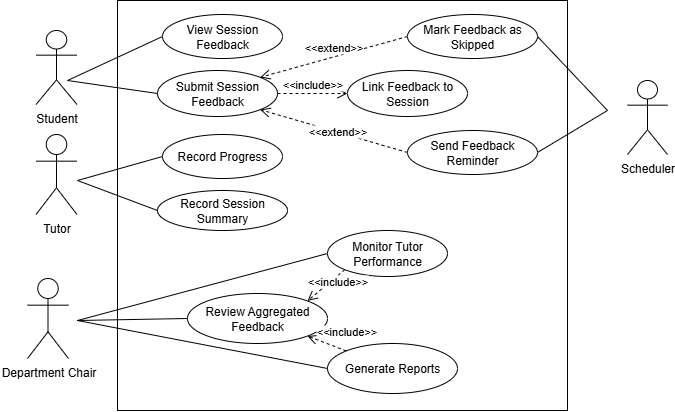
\includegraphics[width=0.9\linewidth]{images/UC-04.png}
\end{center}

\begin{center}
\textbf{Figure 5:}  Submit Session Feedback
\end{center}


\begin{center}
\begin{longtable}{|p{3cm}|p{11cm}|}
\hline
\textbf{Use-case ID} & UC-04a \\ 
\hline
\textbf{Use-case name} & Submit Session Feedback \\ 
\hline
\textbf{Use-case overview} & To allow a student to submit structured feedback after a tutoring session. The feedback is linked to the session and stored for later evaluation and reporting. \\ 
\hline
\textbf{Actors} & 
\begin{itemize}
    \item Student (primary)
    \item Scheduler (secondary, for reminders and marking ‘Skipped’)
\end{itemize} \\ 
\hline
\textbf{Preconditions} & 
\begin{enumerate}
    \item A tutoring session has been completed.
    \item The system is running and accessible.
    \item Student is authenticated in the system.
\end{enumerate} \\ 
\hline
\textbf{Trigger} & The student clicks the ``Submit Feedback'' option after the session is completed. \\ 
\hline
\textbf{Main Flow (Steps)} & 
\begin{enumerate}
    \item System displays a feedback form linked to the completed session.
    \item Student fills in and submits the structured feedback.
    \item System validates the input and saves the feedback in the database.
    \item System links the feedback to the corresponding session.
\end{enumerate} \\ 
\hline
\textbf{Postconditions} & 
\begin{itemize}
    \item Feedback is stored in the database and linked to the correct session.
    \item If skipped, the system records a ``Feedback Skipped'' status for that session.
    \item Data is available for tutors and department chairs in aggregated reports.
\end{itemize} \\ 
\hline
\textbf{Alternative Flows} & 
\begin{itemize}
    \item[AF1] \textbf{Multiple Session Feedback:} If multiple sessions are pending, the system displays a list and allows the student to submit feedback sequentially.
    \item[AF2] \textbf{Draft Save/Connection Loss:} The student may save incomplete feedback as a draft and return later. System automatically saves the draft if connection is lost before final submission.
    \item[AF3] \textbf{Feedback Revision:} Within a defined grace period (e.g., 24h), the student may edit and resubmit feedback; the updated version replaces the original.
    \item[AF4] \textbf{Skipped Feedback:} If no feedback is submitted within the allowed time, the Scheduler triggers a process to mark the session's feedback status as ``Skipped.'' 
\end{itemize} \\ 
\hline
\textbf{Exception Flows} & 
\begin{itemize}
    \item \textbf{Database Error:} If the system fails to save the final submission due to a database error, it logs the error and prompts the student to retry later.
    \item \textbf{Missing Session Record:} If the session record is missing or corrupted, the system logs an error and notifies the coordinator.
\end{itemize} \\ 
\hline
\caption{Use Case UC-04a: Submit Session Feedback}
\end{longtable}
\end{center}

\begin{table}[H]
\centering
\renewcommand{\arraystretch}{1.3}
\begin{tabular}{|p{3cm}|p{11cm}|}
\hline
\textbf{Use-case ID} & UC-04b \\ 
\hline
\textbf{Use-case name} & Record Student Progress \\ 
\hline
\textbf{Overview} & To allow a tutor to record a student’s progress and optionally add a session summary for reference and tracking. \\ 
\hline
\textbf{Actors} & Tutor \\ 
\hline
\textbf{Preconditions} & 
\begin{enumerate}
    \item A tutoring session has been completed.
    \item The system is running and accessible.
    \item Tutor is authenticated in the system.
\end{enumerate} \\ 
\hline
\textbf{Trigger} & Tutor accesses the session record and selects ``Record Progress.'' \\ 
\hline
\textbf{Main Flow (Steps)} & 
\begin{enumerate}
    \item Tutor accesses and opens the specific session record.
    \item Tutor enters progress notes and, optionally, a session summary.
    \item Tutor submits the record.
    \item System validates input and saves the record, linking it to the session.
\end{enumerate} \\ 
\hline
\textbf{Postconditions} & 
\begin{itemize}
    \item Student progress and optional session summary are saved.
    \item Data is linked to the session and available for departmental review.
\end{itemize} \\ 
\hline
\textbf{Alternative Flows} & 
\begin{itemize}
    \item[AF1] \textbf{Optional Summary:} Tutor skips writing a session summary (only progress notes saved).
    \item[AF2] \textbf{Draft Save/Connection Loss:} The tutor may save incomplete notes as a draft and return later. System automatically saves the draft if connection is lost before final submission.
    \item[AF3] \textbf{Note Revision:} Within a defined grace period (e.g., 24h), the tutor may edit and resubmit notes; the updated version replaces the original.
\end{itemize} \\ 
\hline
\textbf{Exception Flows} & 
\begin{itemize}
    \item \textbf{Database Error:} If the system fails to save the record due to a database error, it logs the error and notifies the tutor to retry.
    \item \textbf{Missing/Locked Session:} If the session record is missing or locked by another process, the system notifies the tutor and logs the error.
\end{itemize} \\ 
\hline
\end{tabular}
\caption{Use Case UC-04b: Record Student Progress}
\end{table}

\begin{table}[H]
\centering
\renewcommand{\arraystretch}{1.3}
\begin{tabular}{|p{3cm}|p{11cm}|}
\hline
\textbf{Use-case ID} & UC-04c \\ 
\hline
\textbf{Use-case name} & Review Aggregated Reports (Feedback \& Progress) \\ 
\hline
\textbf{Overview} & To allow the department chair to review aggregated feedback and progress data for monitoring tutor performance and program effectiveness. \\ 
\hline
\textbf{Actors} & Department Chair \\ 
\hline
\textbf{Preconditions} & 
\begin{enumerate}
    \item Feedback and progress records exist in the database.
    \item The system is running and accessible.
    \item Department Chair is authenticated in the system.
\end{enumerate} \\ 
\hline
\textbf{Trigger} & Department Chair selects ``Aggregated Reports Overview.'' \\ 
\hline
\textbf{Main Flow (Steps)} & 
\begin{enumerate}
    \item Department Chair selects report criteria (e.g., date range, tutor, course).
    \item System retrieves all relevant feedback and progress data.
    \item System processes and displays aggregated statistics, charts, or reports.
\end{enumerate} \\ 
\hline
\textbf{Postconditions} & 
\begin{itemize}
    \item Aggregated data is available for decision-making.
    \item Reports may be exported or stored for institutional use.
\end{itemize} \\ 
\hline
\textbf{Alternative Flows} & 
\begin{itemize}
    \item[AF1] \textbf{Filtering:} Department Chair filters or drills down data by tutor, course, or specific time period.
    \item[AF2] \textbf{Export Report:} Department Chair exports the report in a chosen format (e.g., PDF, CSV) for external analysis.
\end{itemize} \\ 
\hline
\textbf{Exception Flows} & 
\begin{itemize}
    \item \textbf{Database/Retrieval Failure:} If database retrieval fails, the system shows a technical error message and logs the issue for system administrators.
    \item \textbf{No Data:} If no data matches the selected criteria, the system displays a clear message: ``No data available for this selection.''
\end{itemize} \\ 
\hline
\end{tabular}
\caption{Use Case UC-04c: Review Aggregated Reports}
\end{table}




% \begin{center}
% 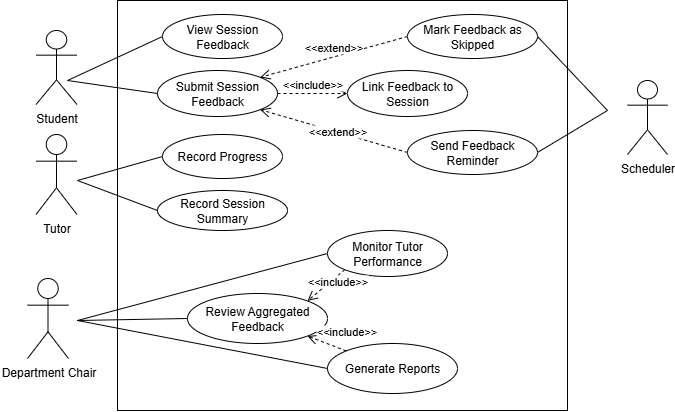
\includegraphics[width=0.9\linewidth]{images/UC-04.png}
% \end{center}

% \begin{center}
% \textbf{Figure 5:}  Submit Session Feedback
% \end{center}


% \begin{table}[h!]
% \centering
% \begin{tabular}{|p{3cm}|p{11cm}|}
% \hline
% \textbf{Use-case ID} & UC-04 \\
% \hline
% \textbf{Use-case name} & Submit Session Feedback \\
% \hline
% \textbf{Use-case overview} & To allow a student to submit structured feedback after a tutoring session. The feedback is linked to the session and stored for later evaluation and reporting. \\
% \hline
% \textbf{Actors} & Student (primary), Scheduler (secondary, for reminders) \\
% \hline
% \textbf{Preconditions} & 
% 1. A tutoring session has been completed. \newline
% 2. The system is running and accessible. \newline
% 3. Student is authenticated in the system. \\
% \hline
% \textbf{Trigger} & The student clicks the ``Submit Feedback'' option after the session is completed. \\
% \hline
% \textbf{Steps} & 
% 1. System displays a feedback form linked to the completed session. \newline
% 2. Student fills in and submits the structured feedback. \newline
% 3. System validates the input and saves the feedback in the database. \newline
% 4. System links the feedback to the corresponding session. \newline
% 5. If no feedback is submitted within the allowed time, the Scheduler triggers reminders. \newline
% 6. If the deadline passes without submission, the system marks the feedback as ``Skipped.'' \\
% \hline
% \textbf{Postconditions} & 
% 1. Feedback is stored in the database and linked to the correct session. \newline
% 2. If skipped, the system records a ``Feedback Skipped'' status for that session. \newline
% 3. Data is available for tutors and department chairs in aggregated reports. \\
% \hline
% \textbf{Alternative Flows} & 
% 1. Multiple Session Feedback → If multiple sessions are pending, the system displays a list and allows the student to submit feedback sequentially. \newline
% 2. Draft Save → The student may save incomplete feedback as a draft and return later within the allowed timeframe. \newline
% 3. Feedback Revision → Within 24h, the student may edit and resubmit feedback; the updated version replaces the original record. \\
% \hline
% \textbf{Exception Flow} & 
% 1. If the student loses connection before submission, the system prompts the student to retry. \newline
% 2. If the session record is missing or corrupted, the system logs an error and notifies the coordinator. \\
% \hline
% \end{tabular}
% \caption{Use Case UC-04: Submit Session Feedback}
% \end{table}